% !TEX root = ../../Dissertation.tex

\begin{refsection}

\chapter[Dichromium oxide \ch{C\lowercase{r}2O2}]{Multireference Characters and Energetic Degeneracy in \ch{Cr2O2^{-/0}}} \label{Cr2O2}


\definecolor{shadecolor}{gray}{0.85}
\begin{shaded}
\textbf{This chapter is based on the paper:}\\
Pham, L. N.; Nguyen, M. T. Another Look at Photoelectron Spectra of the Anion \ch{Cr2O2-}: Multireference Character and Energetic Degeneracy.  \textit{J. Chem. Theory Comput.} \textbf{2018}, 14, 4833–4843. \textit{Reprinted with permission from Journal of Chemical Theory and Computation. Copyright 2018. American Chemical Society.} \textcolor{blue}{\href{https://pubs.acs.org/doi/suppl/10.1021/acs.jctc.8b00412/suppl_file/ct8b00412_si_001.pdf}{The Supporting Information is available online}}.

\emph{My contribution to this work was theoretical calculations, data analysis, discussion, writing of the first draft and revision.}
\newpage
\end{shaded}


\section{Introduction}


With several applications in industry\cite{lunk15,mcdaniel10} and chemical reactions as catalysts,\cite{Rivalta06,Maeda07,zhang09} chromium oxides have been widely studied. Many new chromium oxide clusters were synthesized,\cite{Tono2003B, Tono2003, Janssens07, banobre03, Gutsev01, Zhai06, Zhai08, George97, Moriyama17} and their properties such as magnetic behaviors, geometrical structures and electronic states were also investigated. \cite{Tono2003B, Tono2003, Reddy99, GutsevCr2On, Veliah98, Janssens07, banobre03, Moriyama17} Several electronic, magnetic, and energetic features of chromium oxides are known to be dependent on chemical compositions and geometrical structures. Therefore, geometries of their lowest-lying states must be accurately identified. For this purpose, calculated results obtained using reliable quantum chemical methods still need to be rechecked by comparison with experimental data such as infrared signals and ionization energies. 




Similar to a large number of clusters containing transition metals, theoretical studies of unsaturated chromium oxides are known to be computationally challenging. In fact, such clusters need to be described by wave functions that can accurately address their inherently strong multireference characters. As a result, specific methods, such as the multireference configuration interaction (\acrshort{mrci}), multiconfigurational complete active space followed by perturbation theory (\acrshort{casscf}/\acrshort{caspt2}), and $n$-electron valence state perturbation theory (\acrshort{nevpt2}), are necessary to recover enough correlation energy. When lower levels of theory (usually single-reference methods) were employed, the results obtained for geometric and electronic structures of chromium oxides were frequently not consistent with each other, leading to confusing conclusions. \cite{Tono2003B, Tono2003, Reddy99, GutsevCr2On, wang10, Veliah98, Zhai06, Li07}  




A case in point in which a typical chromium oxide gives rise to conflicting results is dichromium dioxide (\ch{Cr2O2^{-/0}}). Two independent groups probed the electronic structures and magnetic interactions of \ch{Cr2O2} by using anion photoelectron spectroscopy. \cite{Zhai06, Tono2003B} The anion photoelectron spectra recorded by Wang and co-workers\cite{Zhai06} in general reproduced all four distinguished bands reported previously by Tono et al. \cite{Tono2003B}, and interestingly, two additional clear bands were also observed. \cite{Tono2003B, Zhai06} On the one hand, studies of both groups agreed with each other that both the anionic and neutral clusters \ch{Cr2O2^{-/0}} have high-spin ground states of 10 and 9, respectively, in which two chromium atom sites are ferromagnetically coupled. On the other hand, both reports completely disagreed on the band assignments. In addition to the two above reports, several theoretical reports pointed out low-spin-state (singlet) electronic ground states of \ch{Cr2O2}. \cite{wang10, GutsevCr2On, Reddy00, Veliah98} In contrast, some more recent studies again reached the conclusion of a high-spin ground state (dectet) for \ch{Cr2O2-}. \cite{paul09, GutsevCr2On} Even more surprisingly, the geometrical form of \ch{Cr2O2} determined by Ashman and co-workers \cite{Reddy00}  is not consistent with those given in other reports mentioned. \cite{wang10, GutsevCr2On, Reddy00, Veliah98, Tono2003B}  


As summarized above, although experimental spectra obtained from two studies \cite{Tono2003B, Zhai06} appear quite similar, the band assignments differed completely from each other. Tono et al. \cite{Tono2003B} used energies obtained from density functional theory (\acrshort{dft}) for assignments of the four visible bands noted as X' (1.20 vs. 1.40 eV), X (1.69 vs. 1.80 eV), A (2.52 vs. 2.60 eV), B (2.99 vs. 3.10 eV) or C (3.14 vs. 3.10 eV) as shown in Figure \ref{fig:spectra} \cite{Zhai06} (the first and second values given in parentheses are vertical detachment energies (\acrshort{vde}s) taken from refs \citenum{Zhai06} and \citenum{Tono2003B}, respectively). Wang and co-workers \cite{Zhai06} applied an energetic shift of 0.56 eV to \acrshort{vde}s calculated\cite{Tono2003B} to ascribe all transition bands including two new observed ones (B or C and D (3.81 eV), leading to a complete disregard of the very first band X' located at $\sim$1.20 eV. As a consequence, the identity of the first band (X') with extremely low intensity remains to be determined. While this low-intensity band was believed in ref \citenum{Zhai06} to be raised from a lowly populated isomer, \cite{Zhai06} it was attributed in ref \citenum{Tono2003B} to a transition from a highly populated isomer.\cite{Tono2003B} 


\begin{figure}[htb!]
	\centering
	\includegraphics[width=0.5\textwidth]{spectra.pdf}
	\caption{Anion photoelectron spectra of \ch{Cr2O2^-} at two different photon energies of 266 and 193 nm (reproduced with permission from ref \citenum{Zhai06}, Copyright 2006, AIP Publisher).}
	\label{fig:spectra}
\end{figure}


Overall, correct and reliable conclusions on the most stable isomers, electronic ground states, and ionization processes appearing in the anion photoelectron spectra of \ch{Cr2O2-} are still a matter of debate. In this context, we set out to carry out a set of high-accuracy quantum chemical computations with the aim of reinvestigating the geometrical and electronic structures of both \ch{Cr2O2^{-/0}}. Subsequently, all electronic transitions causing the appearance of bands in the photoelectron spectra of the anion \ch{Cr2O2-} are predicted and assigned. A further step, which is multidimensional Franck-Condon factor simulations of the first two bands with lowest ionization energies, is also conducted to corroborate our band assignments. 




\section{Computational Methods}


Generally, the computational procedure includes three steps involving geometry optimizations, additional energy single-point calculations, and Franck–Condon factor simulations. The \acrshort{rasscf}/\acrshort{raspt2} method was first used to optimize geometries of the oxides in both charge states \ch{Cr2O2^{-/0}}. Single-point electronic energy calculations were subsequently conducted using the density-matrix renormalization group \acrshort{dmrg} method, also followed by second-order perturbation treatment \acrshort{caspt2} and \acrshort{dft} computations using different functionals. The last step involving Franck–Condon simulations was performed on the basis of equilibrium structures and harmonic vibrational frequencies obtained from \acrshort{dft} optimizations. To treat the \ch{Cr2O2^{-/0}} clusters with the \acrshort{rasscf}/\acrshort{raspt2} method, \cite{raspt2} a predefined coordinate system was applied to a particular isomer of \ch{Cr2O2^{-/0}}. The four different isomers considered with their predefined coordinate systems are given in Figure \ref{c6fig:coord}.


\begin{figure}[htbp!]
	\centering
	\includegraphics[width=0.4\textwidth]{Cr2O2-coord}
	\caption{Coordinate systems used for \acrshort{rasscf}/\acrshort{raspt2} calculations of four different \ch{Cr2O2} isomers in both neutral and anionic states.}
	\label{c6fig:coord}
\end{figure}



All \acrshort{rasscf}/\acrshort{raspt2}\cite{raspt2} calculations were conducted using the OpenMolcas program.\cite{molcas} The active space used for generations of \acrshort{rasscf} wave functions consists of three subspaces, noted as RAS1, RAS2, and RAS3. While RAS1 contains all six 2p orbitals of two oxygen atoms, RAS3 has no orbitals. Theoretically, some more virtual orbitals can be added to the RAS3 subspace. For transition metals with a more-than-half-filled 3d shell, a set of additional 4d orbitals should be the first choice to account for the 3d double-shell effect. \cite{doubleshell} The inclusion of such an additional d shell would make our computations harder to get convergence and require higher computing resources. More importantly, all metallic 3d molecular orbitals (\acrshort{mo}s) of \ch{Cr2O2^{-/0}} are singly occupied and unoccupied, and as a result, occupation numbers of all 4d orbitals are negligible. Hence, these 4d \acrshort{mo}s are not important, and RAS3 is kept empty with insignificant sacrifice of accuracy. RAS2 is basically comprised of 12 metallic orbitals arising from two chromium atoms, namely, two 4s orbitals and ten 3d ones. A maximum of two electrons were excited from RAS1 to take further static correlation energy into account. Depending on the charged state of \ch{Cr2O2}, the total number of electrons in the active spaces is 20 (for the neutral) or 21 (for the anion). Two \acrshort{rasscf} calculation schemes can be written in a short way as RAS(20,2,0;6,12,0) and RAS(21,2,0;6,12,0) for the neutral and anionic clusters, respectively. The dynamic correlation energy was subsequently calculated employing second-order perturbation theory on the basis of \acrshort{rasscf} wave functions obtained above. All core orbitals of oxygen (1s) and chromium (3p and inner ones) atoms were not considered in the perturbative step. Because the optimization step can only be performed using numerical gradient evaluations at the \acrshort{raspt2} level, many electronic states of the mentioned isomers were, first, roughly optimized with a small basis set \acrshort{ano}-RCC-VDZ, \cite{ano-cr,ano-oxy} and some selected low-lying states were reoptimized with a larger basis set \acrshort{ano}-RCC-VQZP. \cite{ano-cr, ano-oxy} Energetic minima of optimizations were subsequently confirmed by vibrational calculations. However, due to technical shortcomings, only the totally symmetric vibrational modes with respect to the molecular symmetries (C$_{2v}$ and D$_{2h}$) were obtained at the \acrshort{raspt2} level.





The first result revealed from \acrshort{rasscf} calculations is strong multireference features of the wave functions of the \ch{Cr2O2^{-/0}} systems. Therefore, in order to ensure that the \acrshort{raspt2} computations correctly identified ground and important low-lying states, some \acrshort{dmrg}-\acrshort{caspt2} \cite{dmrg1, dmrg2, dmrg3, dmrg4, dmrg5} single-point calculations were also conducted. Single-point energies of some selected low-lying states were thus calculated employing the previously optimized \acrshort{raspt2} geometries. A larger active space with 28 orbitals including all 2s and 2p ones of two oxygen atoms and 3s, 3p, 3d, and 4s orbitals of two chromium atoms was used for \acrshort{dmrg} calculations. The numbers of electrons in the active space amount to 40 and 41 for the neutral and anionic clusters, respectively. The number of the renormalized state m in all \acrshort{dmrg} calculations was set to $m$ = 2000. It is known that to obtain more accurate energies $m$ needs to be >2000, but the resulting \acrshort{dmrg}-\acrshort{caspt2} calculations become computationally expensive, and they go beyond our computing resources. The correlation energy recovered from \acrshort{caspt2} calculations on the basis of \acrshort{dmrg} wave functions did not include the core orbitals excluded in the \acrshort{dmrg} step. The \acrshort{ano}-RCC-VQZP basis set was used for all \acrshort{dmrg}-\acrshort{caspt2} calculations that were done with the CHEMPS2 code\cite{chemps2} interfaced with the OpenMolcas package.




Dozens of \acrshort{dft} single-point calculations were also conducted using the TPSS\cite{TPSS} and BP86 \cite{xbp86, cbp86} functionals in combination with the correlation-consistent quintuple-$\zeta$ aug-cc-pV5Z (for Cr)\cite{basis-Cr} and cc-pV5Z (for O)\cite{basis-O} basis sets implemented in the Molpro 2015 package.\cite{molpro2012} All single-point energy calculations and \acrshort{raspt2} optimizations took all electron scalar relativistic effects into account by use of the second Douglas–Kroll–Hess Hamiltonian (DKH2). \cite{DKH} As proven elsewhere, the zero-point vibrational energies (\acrshort{zpe}s) insignificantly affect positions of small cluster states on their potential energy hypersurfaces;\cite{ZPE} hence, all energies considered in this work are purely electronic energies without \acrshort{zpe} corrections.




To give more details to and support the photoelectron band assignments, equilibrium geometries and corresponding harmonic vibrational frequencies of four states involved in the first two bands X' and X were calculated analytically using \acrshort{dft} with the TPSS functional in conjunction with the def2-TZVP basis set \cite{def2-basis} available in the Gaussian 09 program.\cite{g09} All obtained information was used to simulate the Franck–Condon factors. The integrals between vibrational wave functions were calculated with the MolFC program. \cite{MolFC} As a side note, optimal geometrical parameters of these four states obtained at this \acrshort{dft} level were compared to those optimized at the \acrshort{raspt2} level (see Table \href{https://pubs.acs.org/doi/suppl/10.1021/acs.jctc.8b00412/suppl_file/ct8b00412_si_001.pdf}{\textcolor{blue}{S3}}) to ensure that the TPSS functional is appropriate for Franck-Condon factor simulations.  

\section{Results and Discussion}


\subsection{Ground-State Identification}

Electronic ground states of both \ch{Cr2O2^{-/0}} clusters were determined after two rounds of optimizations. The results of the first round employing the \acrshort{ano}-RCC-VDZ basis set are collected in Table \href{https://pubs.acs.org/doi/suppl/10.1021/acs.jctc.8b00412/suppl_file/ct8b00412_si_001.pdf}{\textcolor{blue}{S1}} of the \href{https://pubs.acs.org/doi/suppl/10.1021/acs.jctc.8b00412/suppl_file/ct8b00412_si_001.pdf}{\textcolor{blue}{Supporting Information}} (available online). We can rule out all low-spin states as candidates for the ground states of both the neutral and anionic clusters. Some high-spin states of the isomers $\textit{a}$, $\textit{b}$ and $\textit{d}$ (Figure \ref{c6fig:coord}) tended to geometrically converge to the same motif of geometry $\textit{c}$ in Figure \ref{c6fig:coord}, belonging to the D$_{2h}$ point group. Therefore, in the second round of optimizations, only high-spin states of the isomer $c$ with spatial symmetry of D$_{2h}$ were selected for geometry reoptimizations using the larger \acrshort{ano}-RCC-VQZP basis set. 




As mentioned above, all electronic states with spin multiplicities of 8, 9, 10, and 11 were reoptimized using the \acrshort{raspt2} method with the \acrshort{ano}-RCC-VQZP basis set, and their relative energies are given in Table \ref{table:relativeE}. Clearly, the \acrshort{raspt2} method identified a dectet state $^{10}$A$_g$ as the most stable electronic structure of the anionic cluster \ch{Cr2O2-}. Interestingly, another dectet state of \ch{Cr2O2-}, namely, $^{10}$B$_{2g}$, was determined to be energetically very close to $^{10}$A$_g$, being about 0.02 eV less stable than the state $^{10}$A$_g$ computed with the \acrshort{raspt2} method. The \acrshort{raspt2} potential energy curves for the two lowest-lying states of the anionic cluster \ch{Cr2O2-} in Figure \ref{fig:surface} strongly corroborate their degeneracy. Due to the very small difference in energy between two lowest-lying anionic states, \acrshort{dmrg}-\acrshort{caspt2} calculations were carried out, and the results obtained confirmed the \acrshort{raspt2} finding. Additionally, to ensure that \acrshort{zpe} corrections do not affect energetic ordering of these two lowest-lying states, their \acrshort{raspt2} and \acrshort{dmrg}-\acrshort{caspt2} energies corrected with the \acrshort{casscf} and TPSS \acrshort{zpe}s were evaluated (see Table \ref{zpe}). Both states $^{10}$A$_g$ and $^{10}$B$_{2g}$ are nearly degenerate, in which the $^{10}$B$_{2g}$ state is only 0.01 eV energetically higher than the ground state. With \acrshort{dft} methods, the results calculated with the TPSS functional seem to be consistent with the \acrshort{raspt2} and \acrshort{dmrg}-\acrshort{caspt2} methods, whereas the BP86 produced a bit of confusion over the ground state of \ch{Cr2O2-}. Overall, one can conclude that the two high-spin dectet states $^{10}$A$_g$ and $^{10}$B$_{2g}$ are degenerate with a marginal energy difference in favor of the $^{10}$A$_g$ state as the ground state of the anionic cluster \ch{Cr2O2-}.


\begin{figure}[htb!]
	\centering
	\includegraphics[width=0.6\textwidth]{potential-surface.pdf}
	\caption{Potential energy curves for the ground and first excited states of \ch{Cr2O2^{-/0}} along the \ch{Cr-Cr} distance at the \acrshort{raspt2} level.}
	\label{fig:surface}
\end{figure}


\begin{table}[htb!]
	\centering
	\begin{threeparttable}
	\caption{Relative Energies (eV) of All Electronic States with Spin Multiplicities of 8, 9, 10, and 11 Determined Using Different Methods\tnote{(a)}}
	\label{table:relativeE}
	\begin{tabular}{lllcllr}
		\toprule
\multirow{2}{*}{isomer} & \multirow{2}{*}{wt.} & \multirow{2}{*}{state} & \multirow{2}{*}{\begin{tabular}[c]{@{}c@{}}\acrshort{raspt2} geometry (\AA{})\\  r$_{Cr-Cr}$, r$_{Cr-O}$\end{tabular}} & \multicolumn{3}{c}{method} \\ \cmidrule{5-7}
		&        &             &         & \acrshort{raspt2}\tnote{(b)}  & TPSS\tnote{(c)} & BP86\tnote{(c)}  \\
		\midrule
		& 0.26   & $^8$A$_g$        & 2.55, 1.83   & 1.10        &      &       \\
		& 0.08   & $^8$B$_{3u}$     & 2.42, 1.84   & 0.62        &      &       \\
		& 0.09   & $^8$B$_{2u}$     & 2.23, 1.84   & 1.32        &      &       \\
		& 0.10   & $^8$B$_{1g}$     & 2.65, 1.82   & 1.20        &      &       \\
		& 0.10   & $^8$B$_{1u}$     & 2.60, 1.82   & 1.45        &      &       \\
		& 0.14   & $^8$B$_{1g}$     & 2.39, 1.83   & 0.78        &      &       \\
c-anion & 0.16   & $^8$B$_{3g}$     & 2.53, 1.83   & 2.45   	 &      &       \\
		& 0.13   & $^8$A$_u$        & 2.63, 1.81   & 1.24        &      &       \\
		& 0.44   & $^{10}$A$_g$     & 2.57, 1.84   & 0.00 (0.00) & 0.00 & 0.00  \\
		& 0.21   & $^{10}$B$_{3u}$  & 2.54, 1.88   & 1.53        & 1.51 & 1.40  \\
		& 0.36   & $^{10}$B$_{2u}$  & 2.48, 1.86   & 1.26        & 0.84 & 0.70  \\      
		& 0.34   & $^{10}$B$_{1g}$  & 2.48, 1.87   & 1.29        & 1.14 & 1.08  \\
		& 0.96   & $^{10}$B$_{1u}$  & 2.66, 1.85   & 3.47        &      &       \\
		& 0.34   & $^{10}$B$_{2g}$  & 2.45, 1.83   & 0.02 (0.01) & 0.11 & -0.01 \\
		& 0.42   & $^{10}$B$_{3g}$  & 2.25, 1.84   & 2.24        & 0.67 & 0.57  \\
		& 0.34   & $^{10}$A$_u$     & 2.29, 1.92   & 2.28        & 0.96 & 0.99  \\
		\midrule
		& 0.59   & $^9$A$_g$        & 2.56, 1.82   & 1.68 (1.40) & 1.38 & 1.43  \\
		& 0.30   & $^9$B$_{3u}$     & 2.53, 1.87   & 3.13        & 2.41 & 2.41  \\
		& 0.69   & $^9$B$_{2u}$     & 2.39, 1.85   & 3.04        & 1.92 & 2.01  \\
		& 0.32   & $^9$B$_{1g}$     & 2.36, 1.88   & 2.21        & 1.67 & 1.83  \\
		& 0.34   & $^9$B$_{1u}$     & 2.39, 1.90   & 2.90        & 2.41 & 2.50  \\
		& 0.37   & $^9$B$_{2g}$     & 2.45, 1.83   & 1.35 (1.25) & 1.28 & 1.33  \\
		& 0.34   & $^9$B$_{3g}$     & 2.61, 1.83   & 2.42        & 2.18 & 2.25  \\
c-neutral & 0.36 & $^9$A$_u$        & 2.56, 1.84   & 2.81   	 & 2.70 & 2.87  \\
		& 0.41   & $^{11}$A$_g$     & 2.50, 1.93   & 6.46        & 5.70 & 5.83  \\
		& 0.53   & $^{11}$B$_{3u}$  & 2.40, 2.02   & 6.77        & 5.12 & 5.33  \\
		& 0.72   & $^{11}$B$_{2u}$  & 2.66, 2.25   & 5.76        & 4.30 & 4.56  \\
		& 0.65   & $^{11}$B$_{1g}$  & 2.45, 2.00   & 5.97        & 4.49 & 4.73  \\
		& 0.60   & $^{11}$B$_{1u}$  & 2.90, 1.90   & 7.52        & 6.03 & 6.24  \\
		& 0.46   & $^{11}$B$_{2g}$  & 2.58, 1.91   & 5.99        & 4.37 & 4.50  \\
		& 0.80   & $^{11}$B$_{3g}$  & 2.51, 2.19   & 6.78        & 5.91 & 6.13  \\
		& 0.40   & $^{11}$A$_u$     & 2.51, 1.93   & 6.59        & 6.05 & 6.33  \\
		\bottomrule
	\end{tabular}
	 \begin{tablenotes}
	 \item[(a)] Coefficient weights of leading configurations are noted as wt.
	 \item[(b)] Values in parentheses are the \acrshort{dmrg}-\acrshort{caspt2} relative energies.
	 \item[(c)] Because coefficient weights (wt.) of some octet states are too small, their \acrshort{dft} energies are not calculated.
	\end{tablenotes}
	\end{threeparttable}
\end{table}


\FloatBarrier

\begin{table}[htb!]
	\centering
	\label{zpe}
	\begin{threeparttable}
	\caption{Insignificant Effects of \acrshort{zpe}s on Energetic Ordering of the Two Lowest Anionic States\tnote{(d)}}
	\begin{tabular}{@{}lcclcclcc@{}}
		\toprule
		\multirow{2}{*}{method} & \multicolumn{2}{c}{without \acrshort{zpe}} &  & \multicolumn{2}{c}{with \acrshort{casscf} \acrshort{zpe}\tnote{(e)}} &  & \multicolumn{2}{c}{with TPSS \acrshort{zpe}} \\ \cmidrule(lr){2-3} \cmidrule(lr){5-6} \cmidrule(l){8-9}  
		             & $^{10}$A$_g$  & $^{10}$B$_{2g}$ &  & $^{10}$A$_g$ & $^{10}$B$_{2g}$ &  & $^{10}$A$_g$  & $^{10}$B$_{2g}$ \\ \midrule 
		\acrshort{raspt2}       & 0.000         & 0.020    &  & 0.000        & 0.022           &  & 0.000         & 0.023           \\
		\acrshort{dmrg}-\acrshort{caspt2}  & 0.000         & 0.010    &  & 0.000        & 0.012           &  & 0.000         & 0.013           \\ \bottomrule
	\end{tabular}
\begin{tablenotes}
	\item[(d)] All relative energies are in eV.
	\item[(e)] To obtain \acrshort{casscf} \acrshort{zpe} values, \acrshort{casscf} calculations were conducted using 12 orbitals (two 4s and ten 3d) only.
\end{tablenotes}
\end{threeparttable}
\end{table}



%TODO The ground state of the neutral cluster

For the neutral cluster, all used methods consistently agree with each other that the $^9$B$_{2g}$ state is the most stable one. The difference in energy of this state with respect to the anionic ground state $^{10}$A$_g$ yielded an adiabatic electron affinity of $\sim$1.30 eV for the neutral oxide. The first excited state of the neutral \ch{Cr2O2} was determined to be the $^9$A$_g$ state at all employed levels of theory. The \acrshort{raspt2} relative energy of this state with respect to the neutral ground state is 0.33 eV, placing it at the first excited position on the potential surface of the neutral \ch{Cr2O2}. The other levels (\acrshort{dmrg}-\acrshort{caspt2}, TPSS, and BP86) estimated that this relative energy is $\sim$0.15 eV.






Our results on the ground state of the anion \ch{Cr2O2-} are in agreement with those of previous reports \cite{Tono2003B}, whereas the ground state $^9$B$_{2g}$ of the neutral is completely different from that given in the same report ($^9$A$_g$).\cite{Tono2003B} In a recent work, \cite{GutsevCr2On} the neutral ground state was identified using \acrshort{dft} computations to have a low-spin multiplicity of 1 (singlet state), which is totally different from our present results. For the anion, the difference becomes more significant because a twisted geometrical chain of the anion \ch{Cr2O2-} was found in ref \citenum{GutsevCr2On} to be the most stable one. \cite{GutsevCr2On} Such an inconsistency in the most stable geometry and electronic ground states can be explained by strong multireference characters of wave functions describing the clusters \ch{Cr2O2^{-/0}}, which can be deduced from the small coefficient weights of the dominant configuration state functions listed in Table \ref{table:relativeE}. These values are around 0.30 -- 0.50 for important states (ground and some excited states involved in the anion photoelectron processes). This suggests that quantum chemical methods with high capability of recovering the static correlation energy are necessary for treatments of \ch{Cr2O2^{-/0}} systems. Single-reference methods are less suitable for the study of \ch{Cr2O2}, resulting in less accurate, if not confusing, results. This is the reason why several \acrshort{dft} studies are not consistent with each other in determination of the geometric and electronic structures of \ch{Cr2O2-} as mentioned above.  



\subsection{Electronic Structures and One-Electron Removals}


The two most stable anionic states $^{10}$A$_g$ and $^{10}$B$_{2g}$ are now analyzed on the basis of their leading electronic configurations extracted from corresponding \acrshort{rasscf} wave functions. Table \ref{table:leadconfig} lists the leading configurations of these two anionic and some selected neutral states. Detailed analysis of the anionic ground state from pseudonatural active orbitals points out that all nine singly occupied orbitals are strongly metallic, in which the 11a$_g$ \acrshort{mo} is mainly composed of the metallic 4s atomic orbitals (\acrshort{ao}s) of chromium atoms and other singly occupied ones originate from 3d \acrshort{ao}s. Within the active space used, there are also six doubly occupied \acrshort{mo}s resulting from six 2p \acrshort{ao}s of the two oxygen atoms. The orbital features of the nearly degenerate state $^{10}$B$_{2g}$ are quite similar to those of the ground state, except for the occupation schemes of two \acrshort{mo}s 2b$_{1g}$ and 4b$_{3g}$. Figure \ref{fig:orb} shows some characteristics of the 18 active-space \acrshort{mo}s of both lowest-lying anionic states.

\begin{figure}[htb!]
	\centering
	\includegraphics[width=\textwidth]{101-106-orbitals.pdf}
	\caption{Pseudonatural orbitals within the active spaces of the ground and first excited states of \ch{Cr2O2-}. In parentheses are the occupation numbers.}
	\label{c6fig:orb}
\end{figure}
 

It is worth noting that from the leading configurations in Table \ref{table:leadconfig} and the electronic features in Figure \ref{c6fig:orb}, one can easily figure out the formal oxidation states of both oxygen and chromium atoms in each state of \ch{Cr2O2^{-/0}}. For example, the anionic ground state $^{10}$A$_g$ has nine singly metallic occupied orbitals and six doubly 2p occupied ones, which means that each oxygen atom captures two electrons and two chromium atoms donate three electrons. Thus, the formal oxidation state of oxygen in the anionic ground state $^{10}$A$_g$ is -2, and that of each chromium atom is +1.5. Formal oxidation states of oxygen and chromium in the anionic $^{10}$B$_{2g}$ state are also -2 and +1.5, respectively. Because one metallic electron is removed from \ch{Cr2O2-} to form the neutral ground state $^9$B$_{2g}$, the formal oxidation state of oxygen is unchanged (-2), and the formal oxidation state of each chromium atom is +2.






Generally, one can divide the 15 occupied orbitals into 3 different types (4s, 3d, and 2p types) depending on their original \acrshort{ao}s. Such origins of orbitals can somehow explain the ionization ordering of \acrshort{mo}s in the photoelectron spectroscopic measurements. With three types of \acrshort{mo}s found, electrons in the 4s-type \acrshort{mo}s are associated with the lowest ionization energy, while the 2p-type \acrshort{mo}s are expected to be at the highest ionization energy. The 3d-type orbitals are in the middle range of ionization energies. This is understandable because for a specific transition metal atom the 4s \acrshort{ao} is energetically higher than 3d orbitals, and as a result, ionization from 4s-type \acrshort{mo}s likely occurs first. Therefore, three ranges of electron signals are expected to be observed in the anion photoelectron spectra of \ch{Cr2O2-}, in which the first and second band regions correspond to electrons removed from the 4s-type and 3d-type \acrshort{mo}s, respectively. The last region of anion photoelectron spectra is expected to be higher in terms of energy because all relevant electrons correspond to higher ionization energies of O(2p) electrons. It should be noted that all predictions are made on the basis of active orbitals constructed and are for a certain upper limit of ionization energy.      

 

\begin{center}
\begin{landscape}
	\small
	\setlength\LTcapwidth{\textwidth} % default: 4in (rather less than \textwidth...)
	\setlength\LTleft{0pt}            % default: \parindent
	\setlength\LTright{0pt}           % default: \fill
\begin{longtable}{@{\extracolsep{\fill}}lllll}
	\caption{Leading Configurations of the Two Most Stable Anionic Ground States and of Neutral Ones. Continuous bands are noted as con.}\\
	\toprule
	state  & wt.     & leading configuration  	  & ionization     & orbital     \\ \midrule 
	\endfirsthead
	\multicolumn{5}{c}%
	{{\tablename\ \thetable{} -- continued from previous page}} \\
	\toprule
	state  & wt.     & leading configuration  	  & ionization     & orbital     \\ \midrule 
	\endhead
	\bottomrule \multicolumn{5}{r}{{Continued on next page}} \\   
	\endfoot	
	\bottomrule 
	\endlastfoot	
	$^{10}$A$_g$     & 0.44 & 8a$_g^2$ 9a$_g^1$ 10a$_g^1$ 11a$_g^1$ 3b$_{3u}^2$ 4b$_{3u}^1$ 5b$_{2u}^2$ 6b$_{2u}^0$ 1b$_{1g}^2$ 2b$_{1g}^1$ 6b$_{1u}^2$ 7b$_{1u}^1$ 8b$_{1u}^1$ 9b$_{1u}^0$ 3b$_{2g}^1$ 3b$_{3g}^2$ 4b$_{3g}^0$ 1a$_u^1$ &                &             \\
	$^{10}$B$_{2g}$  & 0.34 & 8a$_g^2$ 9a$_g^1$ 10a$_g^1$ 11a$_g^1$ 3b$_{3u}^2$ 4b$_{3u}^1$ 5b$_{2u}^2$ 6b$_{2u}^0$ 1b$_{1g}^2$ 2b$_{1g}^0$ 6b$_{1u}^2$ 7b$_{1u}^1$ 8b$_{1u}^1$ 9b$_{1u}^0$ 3b$_{2g}^1$ 3b$_{3g}^2$ 4b$_{3g}^1$ 1a$_u^1$ &                &             \\
	1$^9$A$_g$       & 0.59 & 8a$_g^2$ 9a$_g^1$ 10a$_g^1$ 11a$_g^0$ 3b$_{3u}^2$ 4b$_{3u}^1$ 5b$_{2u}^2$ 6b$_{2u}^0$ 1b$_{1g}^2$ 2b$_{1g}^1$ 6b$_{1u}^2$ 7b$_{1u}^1$ 8b$_{1u}^1$ 9b$_{1u}^0$ 3b$_{2g}^1$ 3b$_{3g}^2$ 4b$_{3g}^0$ 1a$_u^1$ & $^{10}$A$_g$    $\longrightarrow$ 1$^9$A$_g$       & 11a$_g$ (X)    \\
	2$^9$A$_g$       & 0.21 & 8a$_g^2$ 9a$_g^0$ 10a$_g^1$ 11a$_g^1$ 3b$_{3u}^2$ 4b$_{3u}^1$ 5b$_{2u}^2$ 6b$_{2u}^0$ 1b$_{1g}^2$ 2b$_{1g}^1$ 6b$_{1u}^2$ 7b$_{1u}^1$ 8b$_{1u}^1$ 9b$_{1u}^0$ 3b$_{2g}^1$ 3b$_{3g}^2$ 4b$_{3g}^0$ 1a$_u^1$ & $^{10}$A$_g$    $\longrightarrow$ 2$^9$A$_g$       & 9a$_g$(C)     \\
	3$^9$A$_g$       & 0.16 & 8a$_g^2$ 9a$_g^1$ 10a$_g^1$ 11a$_g^1$ 3b$_{3u}^2$ 4b$_{3u}^1$ 5b$_{2u}^2$ 6b$_{2u}^0$ 1b$_{1g}^2$ 2b$_{1g}^0$ 6b$_{1u}^2$ 7b$_{1u}^1$ 8b$_{1u}^1$ 9b$_{1u}^0$ 3b$_{2g}^0$ 3b$_{3g}^2$ 4b$_{3g}^1$ 1a$_u^1$ & $^{10}$B$_{2g}$ $\longrightarrow$ 3$^9$A$_g$       & 3b$_{2g}$ (D')   \\
	4$^9$A$_g$       & 0.24 & 8a$_g^2$ 9a$_g^1$ 10a$_g^0$ 11a$_g^1$ 3b$_{3u}^2$ 4b$_{3u}^1$ 5b$_{2u}^2$ 6b$_{2u}^0$ 1b$_{1g}^2$ 2b$_{1g}^1$ 6b$_{1u}^2$ 7b$_{1u}^1$ 8b$_{1u}^1$ 9b$_{1u}^0$ 3b$_{2g}^1$ 3b$_{3g}^2$ 4b$_{3g}^0$ 1a$_u^1$ & $^{10}$A$_g$    $\longrightarrow$ 4$^9$A$_g$       & 10a$_g$ (D)    \\
	1$^9$B$_{3u}$    & 0.22 & 8a$_g^2$ 9a$_g^1$ 10a$_g^1$ 11a$_g^1$ 3b$_{3u}^2$ 4b$_{3u}^0$ 5b$_{2u}^2$ 6b$_{2u}^0$ 1b$_{1g}^2$ 2b$_{1g}^1$ 6b$_{1u}^2$ 7b$_{1u}^1$ 8b$_{1u}^1$ 9b$_{1u}^0$ 3b$_{2g}^1$ 3b$_{3g}^2$ 4b$_{3g}^0$ 1a$_u^1$ & $^{10}$A$_g$    $\longrightarrow$  1$^9$B$_{3u}$    & 4b$_{3u}$ (C)    \\
	2$^9$B$_{3u}$    & 0.22 & 8a$_g^2$ 9a$_g^1$ 10a$_g^1$ 11a$_g^1$ 3b$_{3u}^2$ 4b$_{3u}^1$ 5b$_{2u}^2$ 6b$_{2u}^0$ 1b$_{1g}^2$ 2b$_{1g}^0$ 6b$_{1u}^2$ 7b$_{1u}^1$ 8b$_{1u}^0$ 9b$_{1u}^0$ 3b$_{2g}^1$ 3b$_{3g}^2$ 4b$_{3g}^1$ 1a$_u^1$ & $^{10}$B$_{2g}$  $\longrightarrow$ 2$^9$B$_{3u}$    & 8b$_{1u}$ (B')   \\
	3$^9$B$_{3u}$    & 0.14 & 8a$_g^2$ 9a$_g^1$ 10a$_g^1$ 11a$_g^1$ 3b$_{3u}^2$ 4b$_{3u}^1$ 5b$_{2u}^2$ 6b$_{2u}^0$ 1b$_{1g}^2$ 2b$_{1g}^0$ 6b$_{1u}^2$ 7b$_{1u}^0$ 8b$_{1u}^1$ 9b$_{1u}^0$ 3b$_{2g}^1$ 3b$_{3g}^2$ 4b$_{3g}^1$ 1a$_u^1$ & $^{10}$B$_{2g}$ $\longrightarrow$ 3$^9$B$_{3u}$    & 7b$_{1u}$ (D')   \\
	1$^9$B$_{2u}$    & 0.69 & 8a$_g^2$ 9a$_g^1$ 10a$_g^1$ 11a$_g^0$ 3b$_{3u}^2$ 4b$_{3u}^1$ 5b$_{2u}^2$ 6b$_{2u}^0$ 1b$_{1g}^2$ 2b$_{1g}^1$ 6b$_{1u}^2$ 7b$_{1u}^0$ 8b$_{1u}^1$ 9b$_{1u}^0$ 3b$_{2g}^1$ 3b$_{3g}^2$ 4b$_{3g}^1$ 1a$_u^1$ &                &             \\                    
	2$^9$B$_{2u}$    & 0.36 & 8a$_g^2$ 9a$_g^1$ 10a$_g^1$ 11a$_g^0$ 3b$_{3u}^2$ 4b$_{3u}^1$ 5b$_{2u}^2$ 6b$_{2u}^0$ 1b$_{1g}^2$ 2b$_{1g}^1$ 6b$_{1u}^2$ 7b$_{1u}^1$ 8b$_{1u}^0$ 9b$_{1u}^0$ 3b$_{2g}^1$ 3b$_{3g}^2$ 4b$_{3g}^1$ 1a$_u^1$ &                &             \\                    
	3$^9$B$_{2u}$    & 0.30 & 8a$_g^2$ 9a$_g^1$ 10a$_g^1$ 11a$_g^1$ 3b$_{3u}^2$ 4b$_{3u}^1$ 5b$_{2u}^2$ 6b$_{2u}^0$ 1b$_{1g}^2$ 2b$_{1g}^0$ 6b$_{1u}^2$ 7b$_{1u}^1$ 8b$_{1u}^1$ 9b$_{1u}^0$ 3b$_{2g}^1$ 3b$_{3g}^2$ 4b$_{3g}^1$ 1a$_u^0$ & $^{10}$B$_{2g}$ $\longrightarrow$ 3$^9$B$_{2u}$    & 1a$_u$ (C')    \\
	1$^9$B$_{1g}$    & 0.32 & 8a$_g^2$ 9a$_g^1$ 10a$_g^1$ 11a$_g^1$ 3b$_{3u}^2$ 4b$_{3u}^1$ 5b$_{2u}^2$ 6b$_{2u}^0$ 1b$_{1g}^2$ 2b$_{1g}^0$ 6b$_{1u}^2$ 7b$_{1u}^1$ 8b$_{1u}^1$ 9b$_{1u}^0$ 3b$_{2g}^1$ 3b$_{3g}^2$ 4b$_{3g}^0$ 1a$_u^1$ & $^{10}$A$_g$    $\longrightarrow$ 1$^9$B$_{1g}$    & 2b$_{1g}$ (A)    \\
	2$^9$B$_{1g}$    & 0.32 & 8a$_g^2$ 9a$_g^1$ 10a$_g^1$ 11a$_g^1$ 3b$_{3u}^2$ 4b$_{3u}^1$ 5b$_{2u}^2$ 6b$_{2u}^0$ 1b$_{1g}^2$ 2b$_{1g}^0$ 6b$_{1u}^2$ 7b$_{1u}^1$ 8b$_{1u}^1$ 9b$_{1u}^0$ 3b$_{2g}^1$ 3b$_{3g}^2$ 4b$_{3g}^0$ 1a$_u^1$ & $^{10}$B$_{2g}$ $\longrightarrow$ 2$^9$B$_{1g}$    & 4b$_{3g}$ (A')   \\
	1$^9$B$_{1u}$    & 0.34 & 8a$_g^2$ 9a$_g^1$ 10a$_g^1$ 11a$_g^1$ 3b$_{3u}^2$ 4b$_{3u}^1$ 5b$_{2u}^2$ 6b$_{2u}^0$ 1b$_{1g}^2$ 2b$_{1g}^1$ 6b$_{1u}^2$ 7b$_{1u}^1$ 8b$_{1u}^0$ 9b$_{1u}^0$ 3b$_{2g}^1$ 3b$_{3g}^2$ 4b$_{3g}^0$ 1a$_u^1$ & $^{10}$A$_g$    $\longrightarrow$ 1$^9$B$_{1u}$    & 8b$_{1u}$ (B)    \\
	2$^9$B$_{1u}$    & 0.19 & 8a$_g^2$ 9a$_g^1$ 10a$_g^1$ 11a$_g^1$ 3b$_{3u}^2$ 4b$_{3u}^1$ 5b$_{2u}^2$ 6b$_{2u}^0$ 1b$_{1g}^2$ 2b$_{1g}^1$ 6b$_{1u}^2$ 7b$_{1u}^0$ 8b$_{1u}^1$ 9b$_{1u}^0$ 3b$_{2g}^1$ 3b$_{3g}^2$ 4b$_{3g}^0$ 1a$_u^1$ & $^{10}$A$_g$    $\longrightarrow$ 2$^9$B$_{1u}$    & 7b$_{1u}$ (B)    \\
	3$^9$B$_{1u}$    & 0.19 & 8a$_g^2$ 9a$_g^1$ 10a$_g^1$ 11a$_g^1$ 3b$_{3u}^2$ 4b$_{3u}^0$ 5b$_{2u}^2$ 6b$_{2u}^0$ 1b$_{1g}^2$ 2b$_{1g}^0$ 6b$_{1u}^2$ 7b$_{1u}^1$ 8b$_{1u}^1$ 9b$_{1u}^0$ 3b$_{2g}^1$ 3b$_{3g}^2$ 4b$_{3g}^1$ 1a$_u^1$ & $^{10}$B$_{2g}$ $\longrightarrow$ 3$^9$B$_{1u}$    & 4b$_{3u}$ (D')   \\
	1$^9$B$_{2g}$    & 0.37 & 8a$_g^2$ 9a$_g^1$ 10a$_g^1$ 11a$_g^0$ 3b$_{3u}^2$ 4b$_{3u}^1$ 5b$_{2u}^2$ 6b$_{2u}^0$ 1b$_{1g}^2$ 2b$_{1g}^0$ 6b$_{1u}^2$ 7b$_{1u}^1$ 8b$_{1u}^1$ 9b$_{1u}^0$ 3b$_{2g}^1$ 3b$_{3g}^2$ 4b$_{3g}^1$ 1a$_u^1$ & $^{10}$B$_{2g}$ $\longrightarrow$ 1$^9$B$_{2g}$   & 11a$_g$ (X')   \\
	2$^9$B$_{2g}$    & 0.11 & 8a$_g^2$ 9a$_g^1$ 10a$_g^1$ 11a$_g^1$ 3b$_{3u}^2$ 4b$_{3u}^1$ 5b$_{2u}^2$ 6b$_{2u}^0$ 1b$_{1g}^2$ 2b$_{1g}^1$ 6b$_{1u}^2$ 7b$_{1u}^1$ 8b$_{1u}^1$ 9b$_{1u}^0$ 3b$_{2g}^0$ 3b$_{3g}^2$ 4b$_{3g}^0$ 1a$_u^1$ & $^{10}$A$_g$    $\longrightarrow$ 2$^9$B$_{2g}$    & 3b$_{2g}$  (C)   \\
	3$^9$B$_{2g}$    & 0.14 & 8a$_g^2$ 9a$_g^1$ 10a$_g^0$ 11a$_g^1$ 3b$_{3u}^2$ 4b$_{3u}^1$ 5b$_{2u}^2$ 6b$_{2u}^0$ 1b$_{1g}^2$ 2b$_{1g}^0$ 6b$_{1u}^2$ 7b$_{1u}^1$ 8b$_{1u}^1$ 9b$_{1u}^0$ 3b$_{2g}^1$ 3b$_{3g}^2$ 4b$_{3g}^1$ 1a$_u^1$ & $^{10}$B$_{2g}$ $\longrightarrow$ 3$^9$B$_{2g}$    & 10a$g$ (D')   \\
	4$^9$B$_{2g}$    & 0.17 & 8a$_g^2$ 9a$_g^0$ 10a$_g^1$ 11a$_g^1$ 3b$_{3u}^2$ 4b$_{3u}^1$ 5b$_{2u}^2$ 6b$_{2u}^0$ 1b$_{1g}^2$ 2b$_{1g}^0$ 6b$_{1u}^2$ 7b$_{1u}^1$ 8b$_{1u}^1$ 9b$_{1u}^0$ 3b$_{2g}^1$ 3b$_{3g}^2$ 4b$_{3g}^1$ 1a$_u^1$ & $^{10}$B$_{2g}$ $\longrightarrow$ 4$^9$B$_{2g}$    & 9a$_g$ (D')    \\
	1$^9$B$_{3g}$    & 0.34 & 8a$_g^2$ 9a$_g^1$ 10a$_g^0$ 11a$_g^0$ 3b$_{3u}^2$ 4b$_{3u}^1$ 5b$_{2u}^2$ 6b$_{2u}^0$ 1b$_{1g}^2$ 2b$_{1g}^1$ 6b$_{1u}^2$ 7b$_{1u}^1$ 8b$_{1u}^1$ 9b$_{1u}^0$ 3b$_{2g}^1$ 3b$_{3g}^2$ 4b$_{3g}^1$ 1a$_u^1$ &                &             \\
	1$^9$A$_{u}$    & 0.34 & 8a$_g^2$ 9a$_g^1$ 10a$_g^1$ 11a$_g^0$ 3b$_{3u}^2$ 4b$_{3u}^1$ 5b$_{2u}^2$ 6b$_{2u}^0$ 1b$_{1g}^2$ 2b$_{1g}^0$ 6b$_{1u}^2$ 7b$_{1u}^1$ 8b$_{1u}^1$ 9b$_{1u}^1$ 3b$_{2g}^1$ 3b$_{3g}^2$ 4b$_{3g}^0$ 1a$_u^1$ &                &             \\
	2$^9$A$_{u}$    & 0.15 & 8a$_g^2$ 9a$_g^1$ 10a$_g^0$ 11a$_g^1$ 3b$_{3u}^2$ 4b$_{3u}^0$ 5b$_{2u}^2$ 6b$_{2u}^0$ 1b$_{1g}^2$ 2b$_{1g}^1$ 6b$_{1u}^2$ 7b$_{1u}^1$ 8b$_{1u}^1$ 9b$_{1u}^0$ 3b$_{2g}^1$ 3b$_{3g}^2$ 4b$_{3g}^1$ 1a$_u^1$ &                &             \\
	3$^9$A$_{u}$    & 0.17 & 8a$_g^2$ 9a$_g^0$ 10a$_g^1$ 11a$_g^1$ 3b$_{3u}^2$ 4b$_{3u}^0$ 5b$_{2u}^2$ 6b$_{2u}^0$ 1b$_{1g}^2$ 2b$_{1g}^1$ 6b$_{1u}^2$ 7b$_{1u}^1$ 8b$_{1u}^1$ 9b$_{1u}^0$ 3b$_{2g}^1$ 3b$_{3g}^2$ 4b$_{3g}^1$ 1a$_u^1$ &                &             \\
	4$^9$A$_{u}$    & 0.12 & 8a$_g^2$ 9a$_g^1$ 10a$_g^1$ 11a$_g^1$ 3b$_{3u}^2$ 4b$_{3u}^1$ 5b$_{2u}^2$ 6b$_{2u}^0$ 1b$_{1g}^2$ 2b$_{1g}^1$ 6b$_{1u}^2$ 7b$_{1u}^1$ 8b$_{1u}^1$ 9b$_{1u}^0$ 3b$_{2g}^1$ 3b$_{3g}^2$ 4b$_{3g}^0$ 1a$_u^0$ & $^{10}$A$_g$     $\longrightarrow$ 4$^9$A$_{u}$    & 1a$_u$ (con.)  \\
	1$^{11}$A$_g$    & 0.50 & 8a$_g^1$ 9a$_g^1$ 10a$_g^1$ 11a$_g^1$ 3b$_{3u}^2$ 4b$_{3u}^1$ 5b$_{2u}^2$ 6b$_{2u}^0$ 1b$_{1g}^2$ 2b$_{1g}^1$ 6b$_{1u}^2$ 7b$_{1u}^1$ 8b$_{1u}^1$ 9b$_{1u}^0$ 3b$_{2g}^1$ 3b$_{3g}^2$ 4b$_{3g}^0$ 1a$_u^1$ & $^{10}$A$_g$     $\longrightarrow$  1$^{11}$A$_g$    & 8a$_g$ (con.)  \\
	1$^{11}$B$_{3u}$ & 0.53 & 8a$_g^2$ 9a$_g^1$ 10a$_g^1$ 11a$_g^1$ 3b$_{3u}^1$ 4b$_{3u}^1$ 5b$_{2u}^2$ 6b$_{2u}^0$ 1b$_{1g}^2$ 2b$_{1g}^1$ 6b$_{1u}^2$ 7b$_{1u}^1$ 8b$_{1u}^1$ 9b$_{1u}^0$ 3b$_{2g}^1$ 3b$_{3g}^2$ 4b$_{3g}^0$ 1a$_u^1$ & $^{10}$A$_g$     $\longrightarrow$ 1$^{11}$B$_{3u}$ & 3b$_{3u}$ (con.) \\
	2$^{11}$B$_{3u}$ & 0.18 & 8a$_g^2$ 9a$_g^1$ 10a$_g^1$ 11a$_g^1$ 3b$_{3u}^2$ 4b$_{3u}^1$ 5b$_{2u}^2$ 6b$_{2u}^0$ 1b$_{1g}^2$ 2b$_{1g}^0$ 6b$_{1u}^1$ 7b$_{1u}^1$ 8b$_{1u}^1$ 9b$_{1u}^0$ 3b$_{2g}^1$ 3b$_{3g}^2$ 4b$_{3g}^1$ 1a$_u^1$ & $^{10}$B$_{2g}$  $\longrightarrow$ 2$^{11}$B$_{3u}$ & 6b$_{1u}$ (con.) \\
	1$^{11}$B$_{2u}$ & 0.72 & 8a$_g^2$ 9a$_g^1$ 10a$_g^1$ 11a$_g^1$ 3b$_{3u}^2$ 4b$_{3u}^1$ 5b$_{2u}^1$ 6b$_{2u}^0$ 1b$_{1g}^2$ 2b$_{1g}^1$ 6b$_{1u}^2$ 7b$_{1u}^1$ 8b$_{1u}^1$ 9b$_{1u}^0$ 3b$_{2g}^1$ 3b$_{3g}^2$ 4b$_{3g}^0$ 1a$_u^1$ & $^{10}$A$_g$     $\longrightarrow$ 1$^{11}$B$_{2u}$ & 5b$_{2u}$ (con.) \\
	1$^{11}$B$_{1g}$ & 0.65 & 8a$_g^2$ 9a$_g^1$ 10a$_g^1$ 11a$_g^1$ 3b$_{3u}^2$ 4b$_{3u}^1$ 5b$_{2u}^2$ 6b$_{2u}^0$ 1b$_{1g}^1$ 2b$_{1g}^1$ 6b$_{1u}^2$ 7b$_{1u}^1$ 8b$_{1u}^1$ 9b$_{1u}^0$ 3b$_{2g}^1$ 3b$_{3g}^2$ 4b$_{3g}^0$ 1a$_u^1$ & $^{10}$A$_g$     $\longrightarrow$ 1$^{11}$B$_{1g}$ & 1b$_{1g}$ (con.) \\
	2$^{11}$B$_{1g}$ & 0.33 & 8a$_g^2$ 9a$_g^1$ 10a$_g^1$ 11a$_g^1$ 3b$_{3u}^2$ 4b$_{3u}^1$ 5b$_{2u}^2$ 6b$_{2u}^0$ 1b$_{1g}^2$ 2b$_{1g}^0$ 6b$_{1u}^2$ 7b$_{1u}^1$ 8b$_{1u}^1$ 9b$_{1u}^0$ 3b$_{2g}^1$ 3b$_{3g}^1$ 4b$_{3g}^1$ 1a$_u^1$ & $^{10}$B$_{2g}$  $\longrightarrow$ 2$^{11}$B$_{1g}$ & 3b$_{3g}$ (con.) \\
	1$^{11}$B$_{1u}$ & 0.60 & 8a$_g^2$ 9a$_g^1$ 10a$_g^1$ 11a$_g^1$ 3b$_{3u}^2$ 4b$_{3u}^1$ 5b$_{2u}^2$ 6b$_{2u}^0$ 1b$_{1g}^2$ 2b$_{1g}^1$ 6b$_{1u}^1$ 7b$_{1u}^1$ 8b$_{1u}^1$ 9b$_{1u}^0$ 3b$_{2g}^1$ 3b$_{3g}^2$ 4b$_{3g}^0$ 1a$_u^1$ & $^{10}$A$_g$     $\longrightarrow$ 1$^{11}$B$_{1u}$ & 6b$_{1u}$ (con.) \\
	2$^{11}$B$_{1u}$ & 0.23 & 8a$_g^2$ 9a$_g^1$ 10a$_g^1$ 11a$_g^1$ 3b$_{3u}^1$ 4b$_{3u}^1$ 5b$_{2u}^2$ 6b$_{2u}^0$ 1b$_{1g}^2$ 2b$_{1g}^0$ 6b$_{1u}^2$ 7b$_{1u}^1$ 8b$_{1u}^1$ 9b$_{1u}^0$ 3b$_{2g}^1$ 3b$_{3g}^2$ 4b$_{3g}^1$ 1a$_u^1$ & $^{10}$B$_{2g}$    $\longrightarrow$ 2$^{11}$B$_{1u}$ & 3b$_{3u}$ (con.) \\
	1$^{11}$B$_{2g}$ & 0.19 & 8a$_g^1$ 9a$_g^1$ 10a$_g^1$ 11a$_g^1$ 3b$_{3u}^2$ 4b$_{3u}^1$ 5b$_{2u}^2$ 6b$_{2u}^0$ 1b$_{1g}^2$ 2b$_{1g}^0$ 6b$_{1u}^2$ 7b$_{1u}^1$ 8b$_{1u}^1$ 9b$_{1u}^0$ 3b$_{2g}^1$ 3b$_{3g}^2$ 4b$_{3g}^1$ 1a$_u^1$ & $^{10}$B$_{2g}$    $\longrightarrow$  $^{11}$B$_{2g}$ & 8a$_g$ (con.)  \\
	1$^{11}$B$_{3g}$ & 0.80 & 8a$_g^2$ 9a$_g^1$ 10a$_g^1$ 11a$_g^1$ 3b$_{3u}^2$ 4b$_{3u}^1$ 5b$_{2u}^2$ 6b$_{2u}^0$ 1b$_{1g}^2$ 2b$_{1g}^1$ 6b$_{1u}^2$ 7b$_{1u}^1$ 8b$_{1u}^1$ 9b$_{1u}^0$ 3b$_{2g}^1$ 3b$_{3g}^1$ 4b$_{3g}^0$ 1a$_u^1$ & $^{10}$A$_g$     $\longrightarrow$ 1$^{11}$B$_{3g}$ & 3b$_{3g}$ (con.) \\
	2$^{11}$B$_{3g}$ & 0.28 & 8a$_g^2$ 9a$_g^1$ 10a$_g^1$ 11a$_g^1$ 3b$_{3u}^2$ 4b$_{3u}^1$ 5b$_{2u}^2$ 6b$_{2u}^0$ 1b$_{1g}^1$ 2b$_{1g}^0$ 6b$_{1u}^2$ 7b$_{1u}^1$ 8b$_{1u}^1$ 9b$_{1u}^0$ 3b$_{2g}^1$ 3b$_{3g}^2$ 4b$_{3g}^1$ 1a$_u^1$ & $^{10}$B$_{2g}$  $\longrightarrow$ 2$^{11}$B$_{3g}$ & 1b$_{1g}$ (con.)\\
	1$^{11}$A$_{u}$ & 0.40 & 8a$_g^2$ 9a$_g^1$ 10a$_g^1$ 11a$_g^1$ 3b$_{3u}^2$ 4b$_{3u}^1$ 5b$_{2u}^1$ 6b$_{2u}^0$ 1b$_{1g}^2$ 2b$_{1g}^0$ 6b$_{1u}^2$ 7b$_{1u}^1$ 8b$_{1u}^1$ 9b$_{1u}^0$ 3b$_{2g}^1$ 3b$_{3g}^2$ 4b$_{3g}^1$ 1a$_u^1$ & $^{10}$B$_{2g}$  $\longrightarrow$  $^{11}$A$_{u}$ & 5b$_{2u}$ (con.)
	\label{table:leadconfig}
\end{longtable}                                                                          
\end{landscape}
\end{center}





In an anion photoelectron spectrum, the strongest bands in the spectra are caused by removal of electrons from an anionic ground state. Let us stress again that in this analysis all inner core orbitals of \ch{Cr2O2-} were not considered. A close look at the leading configurations of the anionic ground state ($^{10}$A$_g$) in Table \ref{table:leadconfig} reveals all possible one-electron removals. In detail, 9 singly occupied orbitals (9a$_g$, 10$a_g$, 11a$_g$, 4b$_{3u}$, 2b$_{1g}$, 7b$_{1u}$, 8b$_{1u}$, 3b$_{2g}$, and 1a$_u$) ionized at relatively low energy and 6 doubly occupied counterparts (8a$_g$, 3b$_{3u}$, 5b$_{2u}$, 1b$_{1g}$, 6b$_{1u}$, and 3b$_{3g}$) with higher one-electron removal energy give rise to 15 ionization processes. Because all ionization processes originate from the most populated anionic ground state $^{10}$A$_g$ of the anion, they should all be observed in the anion photoelectron spectra of \ch{Cr2O2-}. 





As the $^{10}$B$_{2g}$ state is very close to the anionic ground state in terms of its relative energy, this state will have a significant population. Thus, one-electron removals from this nearly degenerate state can also give rise to observed bands in the experimental spectra. This phenomenon was observed elsewhere. \cite{Nhan-vc2, Nhan-tige2} Taking into account all occupied \acrshort{mo}s of the $^{10}$B$_{2g}$ state, another set of 15 orbitals can be equally ionized under a relevant energy of laser beams. Because these 15 ionization processes are predicted to start from a formal excited state, their signals are also predicted to be relatively lower in comparison to those from the anionic ground state. This means that some weak signals can be seen if the experimental spectra are well resolved. Also, these signals can be overshadowed by signals of electrons removed from the ground state or even by the noise. For the sake of understanding, 30 ionization processes and corresponding ionized \acrshort{mo}s are given in Table \ref{table:leadconfig}, in which the coefficient weights of several final neutral states are also collected, which will be analyzed in a following section on the low-intensity bands caused by electrons of the ground state. 

%TODO Oxydation state of anionic and neutral ground states.



\subsection{Anion Photoelectron Spectra}

%TODO Talk a bit about the experimetal bands: how many regions, intensity of bands (band X)

The anion photoelectron spectra of \ch{Cr2O2-} recorded at four photon beam energies \cite{Zhai06} (two of them are provided in Figure \ref{fig:spectra}) look more complicated than those measured earlier. \cite{Tono2003B} In the earlier report,\cite{Tono2003B} two energetic regions of electron signals, in which one region is below 2.0 eV and the other one is over 2.5 eV, were recorded. In the more recent report, one more continuous region over 4.0 eV is present (see Figure \ref{fig:spectra}). \cite{Zhai06} As predicted above, electron removals from three different types of orbitals can give signals to the anion spectra. Obviously, ionization from these three types of \acrshort{mo}s are completely reflected by the observation of three visible regions of signals in the experimental spectra of \ch{Cr2O2-}. \cite{Zhai06} This also implies that the active spaces used in our \acrshort{rasscf} calculations are sufficient to allow us to assign all visible bands.  

%TODO Working point 

In the range of under 2.00 eV, starting from the anionic ground state $^{10}$A$_g$, one electronic transition $^{10}$A$_g$ $\longrightarrow$ 1$^9$A$_g$ was predicted at the \acrshort{raspt2} level. The $^{10}$A$_g$ $\longrightarrow$ 1$^9$A$_g$ \acrshort{vde} and \acrshort{ade} were determined to both be 1.68 eV, which corresponds to the X band with its experimental \acrshort{vde} and \acrshort{ade} of 1.69 and 1.65 eV, respectively (see Table \ref{table:DE}). In this range of ionization energy, starting from the first excited state $^{10}$B$_{2g}$, one more ionization $^{10}$B$_{2g}$ $\longrightarrow$ 1$^9$B$_{2g}$ was found. The calculated \acrshort{vde} of this electronic transition is 1.35 eV. The experimental spectra recorded one band at around 1.20–1.40 eV, noted as X' in Table \ref{table:DE} and in Figure \ref{fig:spectra}. Therefore, this band can be energetically ascribed to the $^{10}$B$_{2g}$ $\longrightarrow$ 1$^9$B$_{2g}$ transition. 


One more interesting fact that further supports such assignments for the first two bands is the relative intensities between two experimental bands in the spectra. The X' band is much less intense as compared to the X band. This suggests that the X' band is likely caused by an experimentally less populated electronic state. Indeed, the $^{10}$B$_{2g}$ $\longrightarrow$ 1$^9$B$_{2g}$ transition originates from the first excited state $^{10}$B$_{2g}$, which may have, according to Maxwell–Boltzmann statistics, $\sim$10\% of probability populated in the ionization region of the spectrometer at 110 K, \cite{Tono2003B} the lowest temperature of the cluster-growth room reported in ref \citenum{Tono2003B}. As a result, all ionization signals coming from this anionic excited state are expected to be lower in intensity, and this is probably what happened to the X' band. To make all electronic transitions starting from the first anionic excited state $^{10}$B$_{2g}$ clear with regard to band assignments, corresponding bands are noted with the prime symbol in Table \ref{table:DE}.    




\begin{table}[htbp!]
	\centering
	\begin{threeparttable}
	\caption{\acrshort{raspt2} \acrshort{ade} and \acrshort{vde} Values of Electronic Transitions Starting from the Nearly Degenerate Anionic States\tnote{(f)}}
	\label{table:DE}

	\begin{tabular}{@{}lllllll@{}}
  \toprule
 \multirow{2}{*}{state} & \multirow{2}{*}{\acrshort{ade} (eV)} & \multirow{2}{*}{\acrshort{vde} (eV)} & \multicolumn{2}{c}{expt. \acrshort{vde} (eV)} & \multirow{2}{*}{band\tnote{(h)}} & \multirow{2}{*}{ionization}  \\ \cmidrule(lr){4-5}
 					 &         &        & ref \citenum{Zhai06}\tnote{(g)}  	 &  ref \citenum{Tono2003B}  &      &                   \\ \midrule
 1$^9$A$_g$          & 1.68    & 1.68   & 1.69 (1.65)& 1.80   & X    & $^{10}$A$_g$    $\longrightarrow$ 1$^9$A$_g$         \\
 2$^9$A$_g$          &         & 3.16   & 3.16       & 3.10   & C    & $^{10}$A$_g$    $\longrightarrow$ 2$^9$A$_g$         \\
 3$^9$A$_g$          &         & 3.88   & 3.81       &        & D'   & $^{10}$B$_{2g}$ $\longrightarrow$ 3$^9$A$_g$         \\
 4$^9$A$_g$          &         & 4.06   & 3.81       &        & D    & $^{10}$A$_g$    $\longrightarrow$ 4$^9$A$_g$         \\
 1$^9$B$_{3u}$       & 2.67    & 3.02   & 3.16       & 3.10   & C    & $^{10}$A$_g$    $\longrightarrow$ 1$^9$B$_{3u}$      \\
 2$^9$B$_{3u}$       &         & 2.90   & 2.99       & 3.10   & B'   & $^{10}$B$_{2g}$  $\longrightarrow$ 2$^9$B$_{3u}$     \\
 3$^9$B$_{3u}$       &         & 3.97   & 3.81       &        & D'   & $^{10}$B$_{2g}$ $\longrightarrow$ 3$^9$B$_{3u}$      \\
 1$^9$B$_{2u}$       &         & 3.04   &            &        &      &                									   \\
 2$^9$B$_{2u}$       &         & 3.11   &            &        &      &                									   \\
 3$^9$B$_{2u}$       &         & 3.33   & 3.16       & 3.10   & C'   & $^{10}$B$_{2g}$ $\longrightarrow$ 3$^9$B$_{2u}$      \\
 1$^9$B$_{1g}$       & 2.22    & 2.41   & 2.52       & 2.60   & A    & $^{10}$A$_g$    $\longrightarrow$ 1$^9$B$_{1g}$      \\
 2$^9$B$_{1g}$       & 2.18    & 2.49   & 2.52       & 2.60   & A'   & $^{10}$B$_{2g}$ $\longrightarrow$ 2$^9$B$_{1g}$      \\
 1$^9$B$_{1u}$       & 2.9     & 2.93   & 2.99       & 3.10   & B    & $^{10}$A$_g$    $\longrightarrow$ 1$^9$B$_{1u}$      \\
 2$^9$B$_{1u}$       &         & 3.01   & 2.99       & 3.10   & B    & $^{10}$A$_g$    $\longrightarrow$ 2$^9$B$_{1u}$      \\
 3$^9$B$_{1u}$       &         & 3.78   & 3.81       &        & D'   & $^{10}$B$_{2g}$ $\longrightarrow$ 3$^9$B$_{1u}$      \\
 1$^9$B$_{2g}$       & 1.35    & 1.35   & 1.20       & 1.40   & X'   & $^{10}$B$_{2g}$ $\longrightarrow$ 1$^9$B$_{2g}$      \\
 2$^9$B$_{2g}$       &         & 3.21   & 3.16       & 3.10   & C    & $^{10}$A$_g$    $\longrightarrow$ 2$^9$B$_{2g}$      \\
 3$^9$B$_{2g}$       &         & 3.58   & 3.81       &        & D'   & $^{10}$B$_{2g}$ $\longrightarrow$ 3$^9$B$_{2g}$      \\
 4$^9$B$_{2g}$       &         & 4.06   & 3.81       &        & D'   & $^{10}$B$_{2g}$ $\longrightarrow$ 4$^9$B$_{2g}$      \\
 1$^9$B$_{3g}$       & 2.42    & 2.66   &            &        &      &                									   \\
 1$^9$A$_u$          & 2.81    & 3.25   &            &        &      &                									   \\
 2$^9$A$_u$          &         & 3.37   &            &        &      &                									   \\
 3$^9$A$_u$          &         & 4.38   &            &        &      &                									   \\
 4$^9$A$_u$          &         & 4.53   & > 4.00     &        & con. & $^{10}$A$_g$     $\longrightarrow$ 4$^9$A$_u$     \\
 1$^{11}$A$_g$       &         & 7.69   & > 4.00     &        & con. & $^{10}$A$_g$     $\longrightarrow$ 1$^{11}$A$_g$     \\
 1$^{11}$B$_{3u}$    & 6.77    & 7.07   & > 4.00     &        & con. & $^{10}$A$_g$     $\longrightarrow$ 1$^{11}$B$_{3u}$  \\
 2$^{11}$B$_{3u}$    &         & 8.49   & > 4.00     &        & con. & $^{10}$B$_{2g}$  $\longrightarrow$ 2$^{11}$B$_{3u}$  \\
 1$^{11}$B$_{2u}$    & 5.76    & 6.66   & > 4.00     &        & con. & $^{10}$A$_g$     $\longrightarrow$ 1$^{11}$B$_{2u}$  \\
 1$^{11}$B$_{1g}$    & 5.97    & 6.36   & > 4.00     &        & con. & $^{10}$A$_g$     $\longrightarrow$ 1$^{11}$B$_{1g}$  \\
 2$^{11}$B$_{1g}$    &         & 8.15   & > 4.00     &        & con. & $^{10}$B$_{2g}$  $\longrightarrow$ 2$^{11}$B$_{1g}$  \\
 1$^{11}$B$_{1u}$    & 7.52    & 7.78   & > 4.00     &        & con. & $^{10}$A$_g$     $\longrightarrow$ 1$^{11}$B$_{1u}$  \\
 2$^{11}$B$_{1u}$    &         & 7.76   & > 4.00     &        & con. & $^{10}$B$_{2g}$  $\longrightarrow$ 2$^{11}$B$_{1u}$  \\
 1$^{11}$B$_{2g}$    &         & 8.25   & > 4.00     &        & con. & $^{10}$B$_{2g}$  $\longrightarrow$ 1$^{11}$B$_{2g}$  \\
 1$^{11}$B$_{3g}$    &         & 7.58   & > 4.00     &        & con. & $^{10}$A$_g$     $\longrightarrow$ 1$^{11}$B$_{3g}$  \\
 2$^{11}$B$_{3g}$    &         & 8.09   & > 4.00     &        & con. & $^{10}$B$_{2g}$  $\longrightarrow$ 2$^{11}$B$_{3g}$  \\
 1$^{11}$A$_{u}$     &         & 7.73   & > 4.00     &        & con. & $^{10}$B$_{2g}$  $\longrightarrow$ 1$^{11}$A$_{u}$  \\ \bottomrule
	\end{tabular}
\begin{tablenotes}
	\item[(f)] Formal bands with the prime symbol are due to transitions starting from the state $^{10}$B$_{2g}$.
	\item[(g)] The value in parentheses is the experimental \acrshort{ade}.
	\item[(h)] Continuous bands are noted as con.
\end{tablenotes}
\end{threeparttable}
\end{table}

  %TODO Second region of spectra 2.00 to 4.00 eV
  
The second region ranging from 2.00 to 4.00 eV in the spectra (Figure \ref{fig:spectra}) shows four visible bands, denoted as A, B, C, and D, in which the B and C bands are not well resolved. At first, for the A band, the electronic transition $^{10}$A$_g$ $\longrightarrow$ 1$^9$B$_{1g}$ has a calculated \acrshort{vde} of 2.41 eV, which is $\sim$0.10 eV smaller than the experimental \acrshort{vde} of the A band. The neutral 1$^9$B$_{3g}$  state with a \acrshort{vde} of 2.66 eV energetically matches the band A, but a comparison between the leading configurations of $^{10}$A$_g$  and 1$^9$B$_{3g}$ listed in Table \ref{table:leadconfig} indicates this ionization is not a one-electron process. Hence, the A band is assigned to the $^{10}$A$_g$ $\longrightarrow$ 1$^9$B$_{1g}$ ionization. Let us note that the 2$^9$B$_{1g}$ state, formed by the $^{10}$B$_{2g}$ $\longrightarrow$ 2$^9$B$_{1g}$ ionization process can also be ascribed to the A band in view of its relative energy. However, this ionization is caused by a transition from the first excited state, and therefore, its signal can be overshadowed by ionization processes from the ground state.




Moving on to the next two bands B and C, these bands are energetically quite close to each other, with a difference in energy of $\sim$0.15 eV. Such a difference in energy is too small to make distinguishable band assignments. Thus, the assignments for the B and C bands can be interchangeable within the error bar of the \acrshort{raspt2} method. To assign these two bands, all electronic transitions from the anionic ground state should be considered first. Within the range of experimental \acrshort{vde}s from 2.99 to 3.16 eV, our calculated \acrshort{vde}s show that five ionization processes, namely, $^{10}$A$_g$ $\longrightarrow$ 1$^9$B$_{1u}$, $^{10}$A$_g$ $\longrightarrow$ 2$^9$B$_{1u}$, $^{10}$A$_g$ $\longrightarrow$ 2$^9$A$_g$, $^{10}$A$_g$ $\longrightarrow$ 1$^9$B$_{3u}$, and $^{10}$A$_g$ $\longrightarrow$ 2$^9$B$_{2g}$ from the anionic ground state, can be attributed to these two bands. Each calculated \acrshort{vde} value of these five electronic transitions lies within an energetic range of 2.93 -- 3.21 eV. Electronic transitions corresponding to each band noted as B and C in this region are listed in Table \ref{table:DE}, and the assignments here are in fact totally interchangeable. Besides, two more additional ionization processes $^{10}$B$_{2g}$ $\longrightarrow$ 2$^9$B$_{3u}$ and $^{10}$B$_{2g}$ $\longrightarrow$ 3$^9$B$_{2u}$ arising from two singly occupied 3d-type \acrshort{mo}s of the nearly degenerate state $^{10}$B$_{2g}$ are likely to take place and give rise to lower-intensity bands (noted as B' and C') dominated by the bands B and C.




The last well-resolved band in the anion photoelectron spectra of \ch{Cr2O2-} was centered at $\sim$3.81 eV. Because of its relatively high ionization energy, this band could not be observed in the earlier report, where the limit was set to $\sim$3.20 eV. \cite{Tono2003B} The intensity of this band is obviously lower than those of the X, A, B, and C bands. However, it is much higher than the intensity of the X' band (see Figure \ref{fig:spectra}). Such a relative intensity of the D band suggests that a one-electron transition starting from the ground state $^{10}$A$_g$ may underlie this band. Because the D band vertically lies at 3.81 eV, the $^{10}$A$_g$ $\longrightarrow$ 4$^9$A$_g$ transition with a computed \acrshort{vde} of 4.06 eV seems to be a good candidate to be responsible for this band. Such a predicted \acrshort{vde} slightly overestimates the experimental value, but this is the only energetically appropriate transition in Table \ref{table:DE}. The D band is assigned to the $^{10}$A$_g$ $\longrightarrow$ 4$^9$A$_g$ ionization process. In Table \ref{table:DE}, five electronic transitions starting from the lowly populated state $^{10}$B$_{2g}$ are theoretically found in the range of 3.78 -- 4.06 eV. Although all of them can contribute to the experimental band D, their low intensities would be overshadowed by signals of the $^{10}$A$_g$ $\longrightarrow$ 4$^9$A$_g$ transition. Note that the leading configuration of the final state 4$^9$A$_g$ has a relatively smaller coefficient weight than those of other final states causing X and A bands. Therefore, the intensity of the D band is lower than those of both the X and A bands.  
  
  %TODO The last region with > 4.00 eV

In Figure \ref{fig:spectra}, a continuous region of signals is present at over 4.00 eV. As analyzed above, due to higher ionization energy, these unwell-resolved signals are expected to come from the ionization processes of electrons in 2p-type \acrshort{mo}s. In Table \ref{table:DE}, twelve 2p-type electronic transitions are listed together with their calculated \acrshort{vde}s of above 6.30 eV. All 12 one-electron transitions lead to the high-spin 11-tet states of the neutral \ch{Cr2O2}. In addition, one 3d-type transition ($^{10}$A$_g$ $\longrightarrow$ 4$^9$A$_u$) contributes to the continuous region. The vertical ionization energy of this transition was computed to be 4.53 eV. If the anion photoelectron spectrum of \ch{Cr2O2-} is more resolved, this band is believed to become pronounced and appear more clearly in the spectrum.

%TODO Discuss how asignments before wrong 

Obviously, most of our present band assignments are different from those reported in two previous studies. \cite{Tono2003B, Zhai06} The nearly degenerate state of the anion \ch{Cr2O2-}, causing the extremely low intensity X' band, was not recognized and was completely ignored in these two reports. A detailed comparison of relative energies between the present \acrshort{raspt2} results and those of Tono and co-workers shows that \acrshort{dft} relative energies reported by these authors are significantly underestimated. This tends to explain the remarkable difference in band assignments. Using an empirical energetic shift of 0.56 eV, Wang and co-workers ruled out the $^9$A$_g$ as the final state underlying the X' band identified by Tono et al., but considered the X band, which is in agreement with our present \acrshort{raspt2} assignment for this band. However, such an empirical energy correction seems not completely effective for the remaining bands (see Table \ref{table:DBA}). 



Let us note that the electronic transition, $^{10}$A$_g$ $\longrightarrow$ 1$^9$B$_{3g}$, is not a one-electron process as found in Tono’s report but a two-electron one. A few additional two-electron processes involving electronic transitions from both degenerate anionic states to the unassigned neutral counterparts can be predicted from Table \ref{table:leadconfig}. Two-electron processes usually appear as low-intensity peaks in anion photoelectron spectra. \cite{ScO, UO2,TiO} Because of low intensities, two-electron signals can be overshadowed by strong and well-resolved bands of the same energy regions. If spectra of strong electron correlation anionic systems are well-resolved and no one-electron processes underlie bands in the energy region of two-electron processes, two-electron detachment signals can be seen even clearly like those in the \ch{UO2-} and \ch{Cu-} anion photoelectron spectra reported by Wang and co-workers. \cite{UO2, CuO}      


\begin{table}[htbp!]
	\centering
	\begin{threeparttable}
	\caption{Comparison of Band Assignments from This Work and Two References  \citenum{Zhai06} and \citenum{Tono2003B}\tnote{(i)}}
	\label{table:DBA}
	\begin{tabular}{@{}llll@{}}
		\toprule
		\multirow{2}{*}{band} & \multicolumn{3}{c}{assignment}                \\ \cmidrule(l){2-4}
	 & this work     		  & ref  \citenum{Zhai06}     & ref \citenum{Tono2003B}   \\ \midrule
 X'  & $^{10}$B$_{2g} \longrightarrow$ 1$^9$B$_{2g}$ &               				             & $^{10}$A$_g \longrightarrow 		$1$^9$A$_g$    \\
 X   & $^{10}$A$_g \longrightarrow$ 1$^9$A$_g$       & $^{10}$A$_g \longrightarrow $1$^9$A$_g$   & $^{10}$A$_g \longrightarrow $1$^9$B$_{3g}$ \\
 A   & $^{10}$A$_g \longrightarrow$ 1$^9$B$_{1g}$    & $^{10}$A$_g \longrightarrow $1$^9$B$_{3g}$& $^{10}$A$_g \longrightarrow $1$^9$B$_{3u}$ \\
	 &               						  		 &               				             & $^{10}$A$_g \longrightarrow $1$^9$B$_{1u}$ \\
 B   & $^{10}$A$_g \longrightarrow$ 1$^9$B$_{1u}$    & $^{10}$A$_g \longrightarrow $1$^9$B$_{3u}$&               \\
	 & $^{10}$A$_g \longrightarrow$ 2$^9$B$_{1u}$    & $^{10}$A$_g \longrightarrow $1$^9$B$_{1u}$&               \\
 C   & $^{10}$A$_g \longrightarrow$ 2$^9$A$_g$       & $^{10}$A$_g \longrightarrow$ 2$^9$A$_g$   & $^{10}$A$_g \longrightarrow $1$^9$B$_{2g}$ \\
	 & $^{10}$A$_g \longrightarrow$ 1$^9$B$_{3u}$    &               				             & $^{10}$A$_g \longrightarrow$ 2$^9$B$_{3u}$ \\
	 & $^{10}$A$_g \longrightarrow$ 2$^9$B$_{2g}$    &               				             &               \\
 D   & $^{10}$A$_g \longrightarrow$ 4$^9$A$_g$       & $^{10}$A$_g \longrightarrow $1$^9$B$_{2g}$&               \\
	 &               					             & $^{10}$A$_g \longrightarrow$ 2$^9$B$_{3u}$&               \\
 con.& $^{10}$A$_g \longrightarrow$ 4$^9$A$_u$       &               		        		     &               \\
	 & $^{10}$A$_g \longrightarrow$ 1$^{11}$A$_g$    &               				             &               \\
	 & $^{10}$A$_g \longrightarrow$ 1$^{11}$B$_{3u}$ &               			                 &               \\
	 & $^{10}$A$_g \longrightarrow$ 1$^{11}$B$_{2u}$ &               				             &               \\
	 & $^{10}$A$_g \longrightarrow$ 1$^{11}$B$_{1g}$ &               				             &               \\
	 & $^{10}$A$_g \longrightarrow$ 1$^{11}$B$_{1u}$ &               				             &               \\
	 & $^{10}$A$_g \longrightarrow$ 1$^{11}$B$_{3g}$ &               				             &               \\ \bottomrule
	\end{tabular}
	\begin{tablenotes}
		\item[(i)] All electronic transitions starting from the anionic ground state $^{10}$A$_g$ and one giving rise to the X' band are listed.
	\end{tablenotes}
\end{threeparttable}
\end{table}

\FloatBarrier

\subsection{Franck-Condon Factor Simulations}


To further support the band assignments discussed above and give more details to band progressions, multidimensional Franck–Condon factor simulations were conducted. Because only the harmonic vibrational frequencies of four states involved in the first two bands ($^{10}$A$_g$, $^9$A$_g$, $^{10}$B$_{2g}$, and $^{9}$B$_{2g}$) were accessible from \acrshort{dft} computations, both X' and X bands were simulated. The equilibrium structures and harmonic vibrational frequencies of the involved states are tabulated in the \href{https://pubs.acs.org/doi/suppl/10.1021/acs.jctc.8b00412/suppl_file/ct8b00412_si_001.pdf}{\textcolor{blue}{SI}}. Two simulated bands are presented in Figure \ref{fig:FC}. The intensity of the X band is much higher than that of the X' band, which is in good agreement with the experiment (Figure \ref{fig:FC}). With regard to band broadening, although the simulated bands do not reproduce well the absolute values of band widths, their relative bandwidth is in good correlation with the experiment. The simulation results not only reflect well the experiment in terms of relative intensities and band widths but also confirm the band assignments for these two bands. 

As explained before, the first two bands are the results of one-electron removals from 4s-type \acrshort{mo}s of \ch{Cr2O2-}. Therefore, vibrational modes including vibrations of Cr atoms are expected in the final states. Indeed, all vibrational modes in the insets show harmonic vibrations of Cr atoms. A deeper investigation into the integrals describing the intensity of the band X' indicates significant involvement of the first excited vibrational state of the \ch{Cr–Cr} stretching mode, while for the X band, the results mainly come from 0 to 0 transitions of the same mode.

%\textit{ The \acrshort{raspt2} equilibrium geometries of two states $^{10}$B$_{2g}$, and $^{9}$B$_{2g}$ in Table \ref{table:relativeE} are nearly the same. As a result, the 0-1 transition integral of the Cr-Cr stretching mode causing the X' band is small.}

\begin{figure}[htb!]
	\centering
	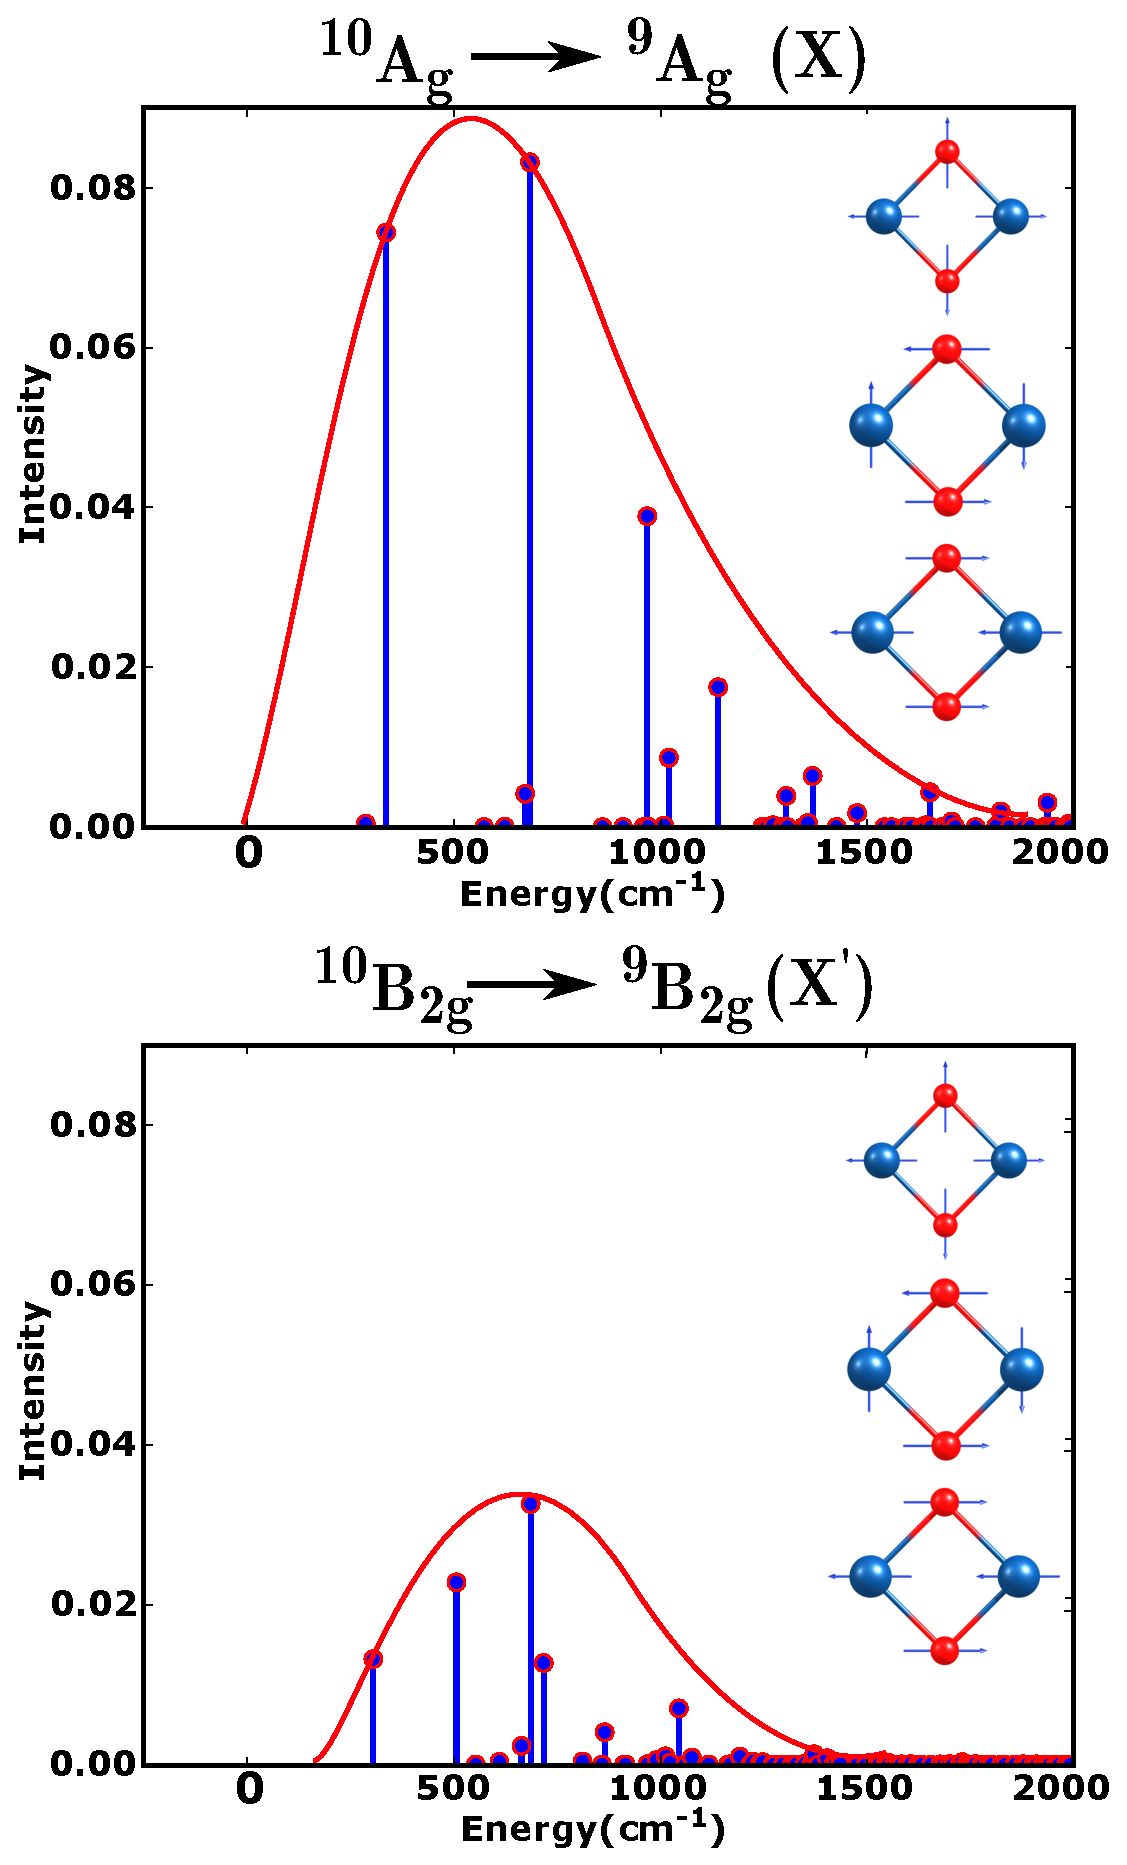
\includegraphics[width=0.5\textwidth]{FC-factor.eps}
	\caption{Franck–Condon factor simulations of the first two bands X' and X in the anion photoelectron spectra of \ch{Cr2O2-}. Vibrational modes obtained from \acrshort{dft} computations giving rise to significant integrals can be seen in the insets.}
	\label{fig:FC}
\end{figure}



\section{Concluding Remarks}



In the present theoretical study, detailed electronic and geometrical structures of the chromium oxides \ch{Cr2O2^{0/-}} were reinvestigated. Geometrical structures of both anionic and neutral clusters of \ch{Cr2O2} have a D$_{2h}$ diamond form. Competition for the anionic ground state of the anion \ch{Cr2O2-} between the two lowest-lying electronic states $^{10}$A$_g$ and $^{10}$B$_{2g}$ was found, in which the $^{10}$A$_g$ state is marginally more stable and within the expected accuracy of the methods employed both states are basically degenerate. 



A high-spin state $^9$B$_{2g}$ is confirmed to be the ground state of the neutral cluster. Both lowest anionic states ($^{10}$A$_g$ and $^{10}$B$_{2g}$) have contributions to the anion photoelectron spectra of the anion \ch{Cr2O2-}. All well-resolved bands with high intensities denoted as X, A, B, C, and D were determined to be the results of one-electron transitions starting from the anionic ground state $^{10}$A$_g$. The lower-intensity X' band is likely caused by the nearly degenerate state $^{10}$B$_{2g}$ when one electron is removed to form the neutral ground state $^9$B$_{2g}$. The degenerate state $^{10}$B$_{2g}$ is also found to undergo several ionization processes and to produce photoelectron signals overshadowed by those originating from the anionic ground state. Overall, most of our spectral assignments for \ch{Cr2O2-} done in this work turn out to be completely different from those given in previous reports. Additionally, band simulations for the first two bands X' and X confirm the anionic ground state and reinforce the band assignments for these two bands.






%%%%%%%%%%%%%%%%%%%%%%%%%%%%%%%%%%%%%%%%%%%%%%%%%%
% Keep the following \cleardoublepage at the end of this file, 
% otherwise \includeonly includes empty pages.
%\cleardoublepage

\includebibliography
\printbibliography[heading=subbibliography] % print section bibliography

\end{refsection}

